Before discussing the previous work on this project, it is important to have a small back-grounder in computer logic. There are primarily two forms of logic (Sequential and Combinational). Sequential logic requires the use of memory elements, this would really restrict the class of algorithms we could test. However, for algorithms that do require extensive use of memory, we will create mixed signal digital-quantum circuits, which can contain memory elements, while also making use of quantum computation. Combinational logic on the other hand does not require memory elements, and simply propagates input values into output responses.



    \begin{wrapfigure}{R}{0.5\textwidth}
   \begin{center}
    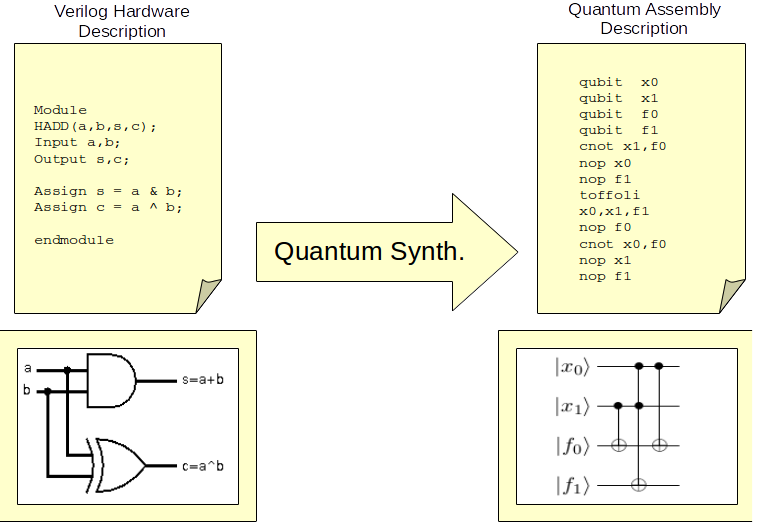
\includegraphics[width=0.40\textwidth]{QuantumSynthesis.png}
  \end{center}
\end{wrapfigure}
One advantage to this project is that a tool which can handle the synthesis of quantum designs given a verilog specification has already been developed. 
As part of the project, this tool will be refined, and utilized to synthesize verilog descriptions of numerical methods into their equivalent quantum forms. 
We will then use an existing quantum simulator to evaluate the speedups that are experienced when using a quantum method for the solution. 
The tool was developed by Micah Thornton, and relies on some previous packages that were developed at other universities such as Berkeley and MIT. 
A pictorial representation of the tool is to the right. 

The diagram represents a purely combinational function, the half-adder, and shows the result of using the tool that has been developed. The boolean functions which represent a half adder are given: 
\begin{center}
$s(a,b) = a \bullet b$
\hspace{5 em}
$c(a,b) = a \oplus b$
\end{center}

By using the quantum synthesis tool we were able to extract the transfer matrix for this logical operation and convert it into a quantum circuit description. This is a very small example, but it illustrates the power of the tool.

This quantum synthesis tool allows us to simply implement the numerical methods in combinational logic and then convert into a quantum assembly definition which can be simulated using any of the wealth of quantum logic simulators readily available online.